\subsection{Challenges in securing EVSE infrastructure}

EVSE infrastructure constitutes a complex system that includes not only charging stations but also sophisticated backend systems and communication protocols. These components and software solutions are typically developed, published, and maintained by various vendors, which makes securing the entire system a challenging task.\\
Combining all the different software from vendors into a secure infrastructure is challenging enough, but the EVSE infrastructure, especially charging stations (CS), is also regularly installed in public places. Even when not in a public setting, these installations are often outdoors, where security measures are significantly lower than in buildings protected by walls, doors, and other physical barriers.\\
In this paper, we focus on wallboxes, which are generally smaller than CS and are typically used in private settings. They are often installed directly on house walls or in garages, and thus still form part of the overall EVSE infrastructure.\\
The fact that they are installed in private areas initially suggests a higher level of security. However, since these areas are still outdoors, we must assume that there are no additional physical security measures beyond the wallbox itself. Therefore, it is crucial to develop a system that not only protects against software-based attacks, such as Denial-of-Service (DoS) or Distributed Denial-of-Service (DDoS), but also considers other potential attack vectors such as firmware manipulation and unauthorized data interception. In addition, the system must secure the hardware against physical threats like tampering, theft, or other intrusions.\\
In our project, we use wallboxes from the \cite{ReSiLENT} project, provided by \cite{StoehrMobility}. The software is developed by \cite{ChargeIQ} and already includes basic security measures to protect against external threats. This project is also carried out in cooperation with \cite{ASVIN}. In the following section, we will take a closer look at the internal components of the wallbox.\\
\begin{figure}[H]
  \centering
  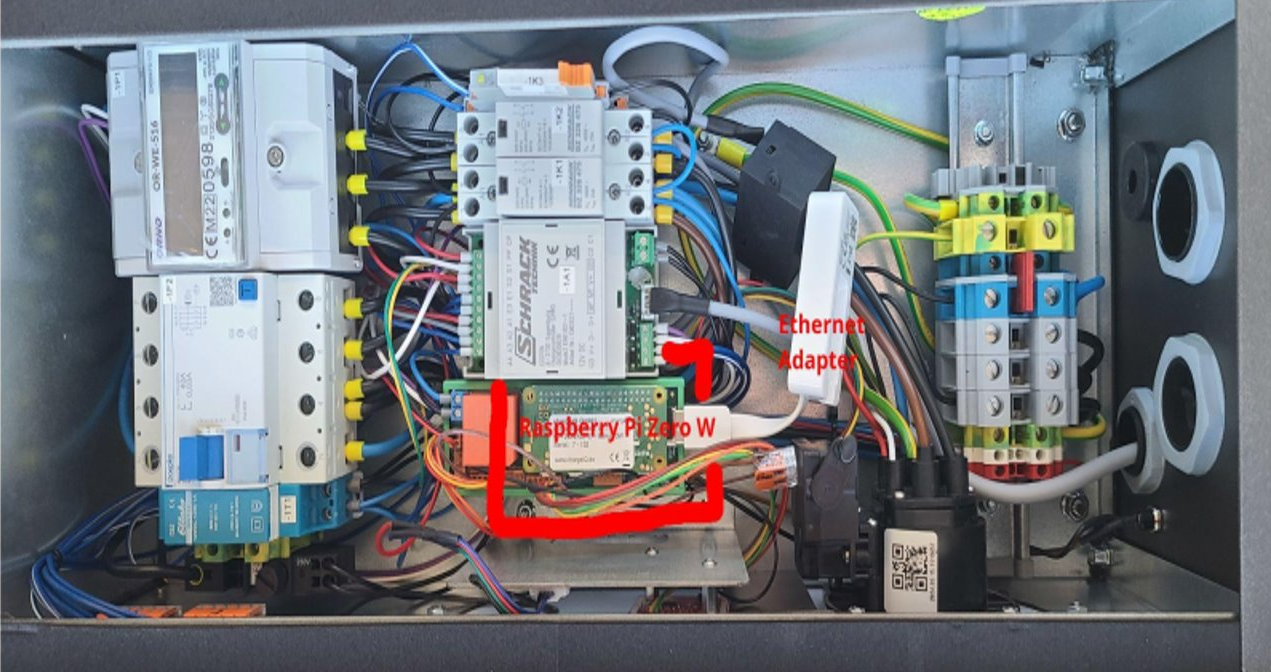
\includegraphics[width=0.7\textwidth]{pics/wallbox.png}
  \caption{Interior view of the wallbox\cite{wallbox}.}
  \label{fig:Wallbox}
\end{figure}
In this figure, the internal components of the wallbox are visible. The wallbox is equipped with a Raspberry Pi Zero W, which serves as the main controller for the planned peer-to-peer communication between the wallboxes. This device is also intended to host of the detection system developed as part of this project.\\
Located behind the Raspberry Pi Zero W is another Raspberry Pi, which is responsible for communication with the backend, including the transmission of user data and handling of payment processes from the Charging process. This component is secured and programmed by \textit{ChargeIQ GmbH}\cite{ChargeIQ}.\\
The sensitive hardware components are enclosed in an aluminum casing designed by \textit{Stöhr Mobility GmbH}\cite{StoehrMobility}, which provides a degree of protection against physical attacks. However, upon closer inspection of these physically secured components, it must be acknowledged that the protective measures can be relatively easily bypassed. This has already been observed and documented by our colleague Lea Laux in her work \cite{Laux2024}.\\
As already mentioned, the wallbox also processes personal data of users, such as their user ID and payment information, in communication with the backend server. This requires special attention in the context of the DSGVO / GDPR, as additional requirements for the protection of personal data like data minimization, storage limitation \cite{DSGVOart5} and legal obligation \cite{DSGVOart6} must be taken into account throughout the entire EVSE infrastructure.\\
Security requires significant computational resources, particularly in the domain of anomaly detection. As shown in Figure~\ref{fig:Wallbox}, the wallbox is equipped with a Raspberry Pi Zero W, which offers relatively sufficient resources for a single-board computer. However, when processing and analyzing over 1,000 hardware events to detect potential anomalies, the system quickly reaches the limits of its hardware capabilities this is just a small example of the challenges we face in securing EVSE infrastructure.\\
Due to the combination of digital and physical threats, the involvement of multiple vendors, and strict data protection requirements, securing Electric Vehicle Supply Equipment (EVSE) infrastructure is a complex task and brings a lot of Challenges.